\chapter{Feuilles d’univers, rotation de Wick et dualité des canaux}

\lectureoverview{Une particule décrit une ligne d’univers ; une corde engendre une feuille d’univers. Quantifier l’un ou l’autre objet exige une somme sur les histoires, mais la somme lorentzienne est oscillante et difficile à définir. En faisant du temps de la feuille d’univers une coordonnée imaginaire, on obtient une théorie euclidienne régie par l’équation de Laplace. Sa symétrie conforme permet alors de transformer la surface fendue d’une interaction entre quatre cordes en un disque portant quatre insertions sur son bord ; la symétrie entre les canaux direct et croisé y devient manifeste.}

\section{De la ligne d’univers à la somme sur les histoires}

Considérons d’abord une particule libre. En mécanique non relativiste, sa position est une fonction \(\mathbf x(t)\) et, en prenant la masse égale à un, son action s’écrit
\begin{equation}
  S_{\mathrm{NR}}[\mathbf x]
  =\frac12\int_{t_1}^{t_2}\dot{\mathbf x}^{\,2}\,dt.
  \label{eq:l07-nr-action}
\end{equation}
Pour une description relativiste, il est plus naturel de réunir le temps et l’espace dans un même vecteur, \(X^\mu(\tau)\), paramétré le long de la trajectoire par \(\tau\). L’expression quadratique correspondante est
\begin{equation}
  S_{\mathrm{rel}}[X]
  =\frac12\int_{\tau_1}^{\tau_2}
  \frac{dX^\mu}{d\tau}\frac{dX_\mu}{d\tau}\,d\tau.
  \label{eq:l07-rel-action}
\end{equation}
Les indices hauts et bas encodent la différence de signe lorentzienne entre le temps et l’espace.
\editorialnote{L’action relativiste quadratique est ici écrite pour une paramétrisation fixée de la ligne d’univers. L’autre possibilité, manifestement invariante par reparamétrisation, est proportionnelle à la longueur propre ; elle sera évoquée plus loin dans le cours.}

\begin{figure}[H]
  \centering
  \includegraphics[width=0.72\textwidth]{lecture_07_figure_01.png}
  \caption{L’action non relativiste et son analogue relativiste quadratique, écrits côte à côte au tableau.}
  \lectureframe{00:03:35}
  \label{fig:l07-particle-actions}
\end{figure}

Classiquement, on fixe les extrémités et on fait varier le chemin. Une particule libre suit alors une ligne d’univers droite, à vitesse constante. La mécanique quantique pose une autre question. Elle ne sélectionne pas une trajectoire unique entre les extrémités : elle demande quelle est l’amplitude pour partir d’un point et être détecté à l’autre. Chaque chemin intermédiaire contribue avec une phase,
\begin{equation}
  K(2,1)=\int_{X(1)}^{X(2)}\!\mathcal D X\,
  e^{iS[X]}.
  \label{eq:l07-feynman-integral}
\end{equation}
L’intégrale fonctionnelle est une intégrale sur un espace de chemins de dimension infinie, et non l’intégrale ordinaire qui figure déjà dans l’action.

\begin{figure}[H]
  \centering
  \includegraphics[width=0.72\textwidth]{lecture_07_figure_02.png}
  \caption{Un chemin représentatif et la phase qui lui est associée avant la somme sur toutes les trajectoires.}
  \lectureframe{00:06:21}
  \label{fig:l07-path-integral-board}
\end{figure}

En langage relativiste, cette amplitude entre deux points est un propagateur. Lors d’une interaction, plusieurs segments de ligne d’univers se rejoignent. On additionne leurs actions, on intègre sur les points de rencontre et on somme les diagrammes comportant les particules externes requises. Ainsi, le développement familier en diagrammes de Feynman est déjà implicitement contenu dans l’instruction de sommer sur les histoires.

Le symbole \(S\) désignera ici une action. Il n’a de lien ni avec l’entropie ni avec la variable de Mandelstam \(s\) utilisée vers la fin du cours. Cette notation commune relève de la tradition plutôt que de la clarté.

\section{Faire pivoter le temps}

\eqref{eq:l07-feynman-integral} pose immédiatement un problème. Chaque facteur \(e^{iS}\) a un module égal à un. Une trajectoire qui oscille de façon désordonnée et la ligne droite classique entrent donc dans la somme avec le même poids en valeur absolue ; seules leurs phases diffèrent. L’interférence destructive permet de retrouver le comportement classique, mais ne transforme pas l’intégrale formelle en un objet ordinaire convergent.

Introduisons un nouveau paramètre \(s\) défini par
\begin{equation}
  \tau=\alpha s,
  \qquad
  d\tau=\alpha\,ds,
  \qquad
  \frac{dX}{d\tau}=\frac{1}{\alpha}\frac{dX}{ds}.
\end{equation}
L’action quadratique se transforme alors comme suit :
\begin{equation}
  \frac12\int d\tau
  \left(\frac{dX}{d\tau}\right)^2
  =
  \frac{1}{2\alpha}\int ds
  \left(\frac{dX}{ds}\right)^2.
  \label{eq:l07-rescaled-action}
\end{equation}
Le choix du contour correspondant à \(\alpha=-i\) transforme le poids oscillant en
\begin{equation}
  e^{iS}
  \longrightarrow
  \exp\!\left[-\frac12\int ds
  \left(\frac{dX}{ds}\right)^2\right]
  =e^{-S_E}.
  \label{eq:l07-euclidean-particle}
\end{equation}

\begin{figure}[H]
  \centering
  \includegraphics[width=0.66\textwidth]{lecture_07_figure_03.png}
  \caption{Le poids euclidien de la particule après la substitution du temps imaginaire ; l’exposant est réel et non positif.}
  \lectureframe{00:16:20}
  \label{fig:l07-particle-wick}
\end{figure}

Un chemin qui s’éloigne beaucoup avant de revenir, ou qui oscille rapidement sans beaucoup se déplacer, a une grande action positive \(S_E\) et est donc exponentiellement supprimé. On obtient une intégrale de type Wiener, pour laquelle il existe une théorie de la convergence rigoureuse. Les extrémités héritées du \(\tau\) réel se trouvent sur un contour \(s\) imaginaire. En pratique, on évalue l’objet euclidien dans son domaine de convergence, puis on prolonge analytiquement le résultat aux variables lorentziennes physiques. C’est la rotation de Wick : pour le calcul, on a fait pivoter le temps, on ne l’a pas supprimé.

\section{Des lignes d’univers aux feuilles d’univers}

Une particule ponctuelle a une ligne d’univers. Une corde ouverte engendre un ruban, et une corde fermée, un tube. Les coordonnées \((\sigma,\tau)\) repèrent les points de cette feuille d’univers bidimensionnelle, tandis que
\begin{equation}
  X^\mu=X^\mu(\sigma,\tau)
  \label{eq:l07-embedding}
\end{equation}
donne la position dans l’espace-temps du point repéré. La connaissance de toutes les fonctions \(X^\mu\) spécifie l’histoire complète de la corde.

L’action quadratique lorentzienne sur la feuille d’univers a la même structure cinétique moins potentiel que celle d’une corde vibrante ordinaire :
\begin{equation}
  S_{\mathrm{ws}}[X]
  =\frac{T_s}{2}\int d\tau\,d\sigma\,
  \left[
    \partial_\tau X^\mu\partial_\tau X_\mu
    -
    \partial_\sigma X^\mu\partial_\sigma X_\mu
  \right].
  \label{eq:l07-lorentzian-worldsheet}
\end{equation}
La tension totale \(T_s\) fixe l’échelle ; le cours la laisse de côté pour se concentrer sur la structure des dérivées.

\begin{figure}[H]
  \centering
  \includegraphics[width=0.72\textwidth]{lecture_07_figure_04.png}
  \caption{L’action lorentzienne sur la feuille d’univers pour \(X^\mu(\sigma,\tau)\), avec son signe cinétique moins potentiel.}
  \lectureframe{00:24:26}
  \label{fig:l07-worldsheet-action}
\end{figure}

On obtient l’amplitude de la corde en exponentiant cette action et en sommant sur toutes les surfaces qui relient les configurations initiale et finale prescrites de la corde :
\begin{equation}
  \mathcal A=\int\mathcal D X\,e^{iS_{\mathrm{ws}}[X]}.
  \label{eq:l07-surface-integral}
\end{equation}
La même règle s’applique à deux cordes qui en deviennent deux, à deux qui en deviennent trois, ou à toute autre configuration externe autorisée. Les différentes topologies de feuilles d’univers font également partie de la somme. Ajouter des trous aux surfaces est l’analogue, pour les cordes, de l’ajout de boucles dans le développement en diagrammes pour les particules ponctuelles.

\begin{figure}[H]
  \centering
  \includegraphics[width=0.66\textwidth]{lecture_07_figure_05.png}
  \caption{Une surface reliant plusieurs cordes externes, avec un trou représentant une topologie différente de la feuille d’univers.}
  \lectureframe{00:27:14}
  \label{fig:l07-surface-topology}
\end{figure}

\begin{classroomqa}\audiencequestion{Pour un électron ponctuel, la dérivée par rapport à \(\sigma\) ne s’annule-t-elle pas tout simplement ? \lecturetimestamp{00:27:56}}\lecturerresponse{Une particule ponctuelle n’a pas de coordonnée \(\sigma\) au départ. Les représentations restent néanmoins liées : lorsque les états externes sont légers par rapport à l’échelle de la corde et que les énergies des processus sont faibles, les amplitudes des cordes reproduisent les diagrammes de Feynman ordinaires des particules ponctuelles. Cette limite ne revient pas simplement à annuler une dérivée.}\end{classroomqa}

L’intégrale sur les surfaces présente le même problème de convergence que l’intégrale sur les chemins. Après rotation de Wick du temps sur la feuille d’univers, sa forme euclidienne stable est
\begin{equation}
  \begin{aligned}
    S_{E,\mathrm{ws}}[X]
    &=\frac{T_s}{2}\int d\tau\,d\sigma\,
      \left[
        \partial_\tau X^\mu\partial_\tau X_\mu
        +\partial_\sigma X^\mu\partial_\sigma X_\mu
      \right],\\
    \mathcal A_E&=\int\mathcal D X\,e^{-S_{E,\mathrm{ws}}}.
  \end{aligned}
  \label{eq:l07-euclidean-worldsheet}
\end{equation}
Les deux dérivées interviennent maintenant avec le même signe positif. Une surface qui vibre violemment ou qui est fortement étirée a une grande action euclidienne et est supprimée.

\begin{figure}[H]
  \centering
  \includegraphics[width=0.72\textwidth]{lecture_07_figure_06.png}
  \caption{La densité euclidienne positive sur la feuille d’univers après la rotation de \(\tau\) vers le temps imaginaire.}
  \lectureframe{00:34:29}
  \label{fig:l07-worldsheet-wick}
\end{figure}

Il existe aussi une formulation géométrique directe. On peut associer à une particule relativiste une action proportionnelle à la longueur propre de son chemin, et à une corde, une action proportionnelle à l’aire dans l’espace-temps de sa feuille d’univers. La seconde est l’action de Nambu--Goto. La forme quadratique sur la feuille d’univers utilisée ici est appelée conventionnellement forme de Polyakov ; elle est bien plus facile à manier pour le calcul présent.
\editorialnote{Le cours comporte une remarque humoristique sur les dénominations historiques et mentionne également l’action de Liouville et les conditions aux limites de Dirichlet. Il n’est pas nécessaire de revendiquer une priorité pour cette dérivation : seule est utilisée l’équivalence entre les formulations en termes d’aire et de métrique auxiliaire.}

\section{L’équation du mouvement euclidienne}

Les coordonnées \(\sigma\) et \(\tau\) ne sont que des repères sur la feuille. La question suivante s’impose donc : quels changements de repères laissent la théorie inchangée ? L’équation du mouvement permet de le voir facilement. En faisant varier \eqref{eq:l07-euclidean-worldsheet}, on obtient, composante par composante,
\begin{equation}
  \partial_\tau^2X^\mu+\partial_\sigma^2X^\mu=0.
  \label{eq:l07-laplace}
\end{equation}
Avant la rotation de Wick, le signe relatif est négatif et il s’agit d’une équation d’onde. En signature euclidienne, les deux signes sont positifs : c’est donc l’équation de Laplace en deux dimensions.

\begin{classroomqa}\audiencequestion{Est-ce l’équation d’un tambour vibrant ?
\lecturetimestamp{00:41:50}}\lecturerresponse{Elle lui est étroitement apparentée, mais un tambour vibrant comporte aussi une coordonnée de temps réel et obéit donc à une équation d’onde. L’équation considérée ici est l’équation de Laplace euclidienne. Le potentiel électrostatique dans une région sans charges en est un exemple familier plus direct.}\end{classroomqa}

\begin{classroomqa}\audiencequestion{L’action contient des dérivées premières. Pourquoi son équation contient-elle des dérivées secondes ? \lecturetimestamp{00:42:44}}\lecturerresponse{Faire varier un terme quadratique en une dérivée première, puis intégrer par parties, revient à déplacer une dérivée sur cette dérivée première. C’est l’analogue, en théorie des champs, du fait que \(\dot x^{\,2}\) dans une action produit \(\ddot x\) dans l’équation du mouvement.}\end{classroomqa}

\begin{figure}[H]
  \centering
  \includegraphics[width=0.68\textwidth]{lecture_07_figure_07.png}
  \caption{L’équation de Laplace avec des signes positifs et la première ligne discrète qui sert à interpréter ses dérivées secondes.}
  \lectureframe{00:43:30}
  \label{fig:l07-laplace-board}
\end{figure}

Pour visualiser la géométrie, discrétisons d’abord une coordonnée avec un pas de \(\epsilon\). Une dérivée première est une différence entre points voisins, tandis qu’une dérivée seconde est une différence entre différences voisines :
\begin{equation}
  \frac{d^2X}{ds^2}\bigg|_{2}
  \longrightarrow
  \frac{X(3)-2X(2)+X(1)}{\epsilon^2}.
  \label{eq:l07-second-difference}
\end{equation}

\begin{figure}[H]
  \centering
  \includegraphics[width=0.72\textwidth]{lecture_07_figure_08.png}
  \caption{La ligne numérotée, un petit morceau de réseau et le développement aux différences finies d’une dérivée seconde.}
  \lectureframe{00:45:51}
  \label{fig:l07-finite-difference-board}
\end{figure}

Discrétisons maintenant le plan \((\sigma,\tau)\). Repérons les quatre plus proches voisins d’un point central \(5\) par \(1,2,3,4\). L’équation
\eqref{eq:l07-laplace} devient
\begin{equation}
  X(1)+X(2)+X(3)+X(4)-4X(5)=0,
\end{equation}
ou encore
\begin{equation}
  X(5)=\frac14\bigl[X(1)+X(2)+X(3)+X(4)\bigr].
  \label{eq:l07-mean-value}
\end{equation}

\begin{figure}[H]
  \centering
  \includegraphics[width=0.72\textwidth]{lecture_07_figure_09.png}
  \caption{L’équation bidimensionnelle aux différences finies obtenue : la valeur au centre est égale à la moyenne de ses quatre voisines.}
  \lectureframe{00:48:26}
  \label{fig:l07-mean-value-board}
\end{figure}

Cette propriété de la valeur moyenne vaut pour un carré infinitésimal quelle que soit son orientation. Elle exprime le contenu géométrique local de l’équation de Laplace et établit le lien avec la symétrie conforme.

\section{Coordonnées conformes}

Considérons un changement de \((\sigma,\tau)\) en \((\sigma',\tau')\). Une déformation générale transforme un petit carré en un quadrilatère quelconque. Les transformations qui nous intéressent ici ont ceci de particulier qu’elles transforment chaque carré infinitésimal en un autre carré infinitésimal, éventuellement tourné et redimensionné. De manière équivalente, elles préservent les angles entre les courbes qui se coupent. Ce sont les transformations conformes.

\begin{figure}[H]
  \centering
  \includegraphics[width=0.68\textwidth]{lecture_07_figure_10.png}
  \caption{Un carré local transformé en une autre petite figure, dont on vérifie la préservation des angles par la transformation conforme.}
  \lectureframe{00:53:25}
  \label{fig:l07-conformal-board}
\end{figure}

\begin{classroomqa}\audiencequestion{Si les angles sont préservés, la transformation se réduit-elle essentiellement à une rotation ? \lecturetimestamp{00:53:31}}\lecturerresponse{Cela n’est vrai que localement ; même localement, un changement d’échelle uniforme est également permis. La rotation et le facteur d’échelle locaux peuvent varier d’un point à l’autre : le réseau de coordonnées peut donc se courber, s’agrandir dans une région et se contracter dans une autre, tout en préservant les formes infinitésimales.}\end{classroomqa}

Une application qui préserve les angles ne préserve pas nécessairement les dimensions. Si celles-ci étaient aussi conservées partout, il ne resterait que la classe bien plus restreinte des transformations rigides : les translations et les rotations. Les applications conformes préservent plutôt la forme locale. C’est pourquoi une projection cartographique peut préserver la forme d’une petite île tout en déformant considérablement son aire.

\begin{classroomqa}\audiencequestion{Une application conforme signifie-t-elle que le système de coordonnées est plat ? \lecturetimestamp{00:55:35}}\lecturerresponse{Non. La platitude et la conformalité sont deux propriétés différentes. Une application conforme peut utiliser des lignes de coordonnées courbes ; elle préserve l’angle entre les courbes qui se coupent. Une projection cartographique de type Mercator est un exemple familier de préservation locale des formes accompagnée d’une forte déformation des échelles.}\end{classroomqa}

En deux dimensions, les transformations requises sont engendrées localement par des fonctions analytiques d’une coordonnée complexe
\begin{equation}
  z=\sigma+i\tau.
\end{equation}
Les frontières finies peuvent changer d’apparence de façon spectaculaire. Une région carrée peut être envoyée sur une région aux contours lisses, les coins initiaux devenant des points ordinaires du nouveau bord plutôt que ses points visuellement les plus saillants. Il n’y a pas de contradiction : la conformalité est une propriété locale à l’intérieur de la région, et l’application préserve les angles infinitésimaux partout où elle est régulière.

\begin{classroomqa}\audiencequestion{Cette liberté de choix des coordonnées explique-t-elle pourquoi le diagramme précédent de jonction--séparation pouvait être choisi symétrique ?
\lecturetimestamp{00:56:32}}\lecturerresponse{Oui. La même liberté conforme qui préserve les équations de la feuille d’univers nous permet de remplacer la bande d’interaction peu commode par un domaine plus symétrique. La liberté restante n’élimine pas le paramètre physique de jonction--séparation ; elle le reformule comme la position relative des insertions sur le bord.}\end{classroomqa}

\section{De la feuille fendue au disque}

Revenons à la diffusion de quatre cordes. Deux cordes ouvertes entrent, leurs extrémités se rejoignent, la corde résultante se propage, puis se sépare. Représenté sur une feuille d’univers plane, le processus forme une bande infinie fendue à chaque extrémité. La distance \(\tau_0\) entre les pointes des fentes est la durée de vie de la corde intermédiaire, et l’amplitude s’intègre sur cette durée.

\begin{figure}[H]
  \centering
  \includegraphics[width=0.72\textwidth]{lecture_07_figure_11.png}
  \caption{La bande à deux fentes représentant la jonction de deux cordes ouvertes, leur propagation commune, puis leur séparation.}
  \lectureframe{01:00:20}
  \label{fig:l07-slit-strip}
\end{figure}

Après euclidisation, les champs d’immersion sur cette région satisfont à l’équation de Laplace. L’invariance conforme permet donc de transformer la bande fendue en disque. On peut se représenter la topologie en feuilletant le disque par des cercles concentriques, puis en déformant continûment ces courbes fermées jusqu’à ce qu’elles remplissent la région fendue. Par l’application, les extrémités à l’infini deviennent des points exceptionnels du bord.

\begin{figure}[H]
  \centering
  \includegraphics[width=0.72\textwidth]{lecture_07_figure_12.png}
  \medskip

  \begin{adjustbox}{max width=\linewidth}
  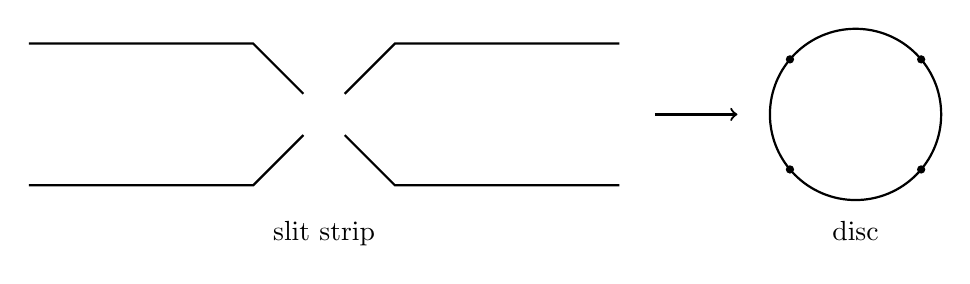
\begin{tikzpicture}[x=0.75cm,y=0.75cm]
    \draw[thick] (-5,1.2) -- (-1.2,1.2) -- (-0.35,0.35);
    \draw[thick] (-5,-1.2) -- (-1.2,-1.2) -- (-0.35,-0.35);
    \draw[thick] (0.35,0.35) -- (1.2,1.2) -- (5,1.2);
    \draw[thick] (0.35,-0.35) -- (1.2,-1.2) -- (5,-1.2);
    \draw[->,thick] (5.6,0) -- (7.0,0);
    \draw[thick] (9.0,0) circle (1.45);
    \foreach \a in {40,140,220,320} \fill (9.0,0) ++(\a:1.45) circle (1.5pt);
    \node[below] at (0,-1.65) {slit strip};
    \node[below] at (9.0,-1.65) {disc};
  \end{tikzpicture}
  \end{adjustbox}
  \caption{Comparaison au tableau des courbes de niveau et schéma clair de l’application conforme de la bande fendue sur un disque. Les quatre extrémités externes deviennent quatre points particuliers du bord.}
  \lectureframe{01:04:46}
  \label{fig:l07-strip-to-disc}
\end{figure}

Les états externes ne disparaissent pas lors de ce changement de coordonnées. Il faut insérer l’impulsion, le type de particule et le niveau d’oscillation aux quatre points exceptionnels. Les objets formels qui portent ces informations sont les opérateurs de vertex. Leur construction détaillée sera présentée plus tard, mais leur rôle est déjà clair : ils transforment une intégrale de chemin sur une feuille d’univers autrement homogène en une expérience de diffusion spécifiée.

Après avoir utilisé les transformations conformes du disque pour placer trois points du bord à des positions de référence commodes, il reste une position relative réelle. On peut la représenter par le birapport des quatre points ordonnés du bord. C’est l’analogue, sur le disque, de l’ancienne durée de vie \(\tau_0\).

\begin{figure}[H]
  \centering
  \includegraphics[width=0.62\textwidth]{lecture_07_figure_13.png}
  \caption{Quatre points d’insertion sur le bord du disque. La liberté conforme élimine tous les degrés de liberté de leur configuration ordonnée, à l’exception d’un module réel.}
  \lectureframe{01:10:55}
  \label{fig:l07-four-points}
\end{figure}

L’intégrale sur la durée de vie n’a donc pas disparu. Elle est devenue une intégrale sur le module restant. Avec la coordonnée conventionnelle \(0<z<1\), l’intégrale à quatre points pour les cordes ouvertes prend la même forme que dans le cours précédent,
\begin{equation}
  \mathcal A(s,t)\propto
  \int_0^1 z^{-s-1}(1-z)^{-t-1}\,dz.
  \label{eq:l07-modulus-integral}
\end{equation}

\section{Deux limites d’une même surface}

À une extrémité de l’espace des modules, les deux points d’insertion associés à la paire entrante se rapprochent. Dans les coordonnées de la bande fendue, cela correspond à un long intervalle entre la jonction et la séparation : une corde intermédiaire du canal direct se propage pendant longtemps. À l’autre extrémité, une autre paire de points voisins se rapproche. On interprète alors naturellement la même surface comme un échange dans le canal croisé. Sur la bande, ces descriptions semblent sans rapport, mais elles correspondent à deux limites voisines du bord de l’intégrale sur le disque.

Revenons à la convention majoritairement positive du cours précédent :
\begin{equation}
  -s=(k_1+k_2)^2,
  \qquad
  -t=(k_1+k_3)^2.
  \label{eq:l07-mandelstam}
\end{equation}
La limite directe organise les pôles en \(s\) ; la limite croisée organise les pôles en \(t\).
\editorialnote{Vers la fin du cours, le tableau utilise une convention de signe abrégée pour les invariants de Mandelstam, tout en identifiant \(s\) à l’énergie au centre de masse au carré, qui est positive. L’équation \eqref{eq:l07-mandelstam} conserve la convention majoritairement positive établie dans le cours 6.}

\begin{figure}[H]
  \centering
  \includegraphics[width=0.62\textwidth]{lecture_07_figure_14.png}
  \caption{Les diagrammes des deux canaux : une longue propagation dans une orientation, et un échange dans l’orientation croisée.}
  \lectureframe{01:19:27}
  \label{fig:l07-channel-diagrams}
\end{figure}

\begin{figure}[H]
  \centering
  \includegraphics[width=0.72\textwidth]{lecture_07_figure_15.png}
  \caption{Le tableau revient aux appariements des impulsions dans les canaux \(s\) et \(t\), en comparant les deux limites du module du disque.}
  \lectureframe{01:19:40}
  \label{fig:l07-st-board}
\end{figure}

Un seul objet analytique fournit donc les deux développements :
\begin{equation}
  \mathcal A(s,t)=\mathcal A(t,s).
\end{equation}
C’est la dualité des canaux. Dans le langage d’origine des résonances, il semblait miraculeux qu’une somme sur les états du canal direct puisse également rendre compte de l’échange dans le canal croisé. Sur la feuille d’univers euclidienne, la symétrie conforme explique pourquoi ces deux descriptions correspondent à une seule et même surface. Historiquement, cette interprétation a suivi de très près la découverte, en 1969, de l’amplitude de Veneziano.

\begin{classroomqa}\audiencequestion{Existe-t-il aussi une représentation en bande fendue correspondant à l’orientation croisée ? \lecturetimestamp{01:20:49}}\lecturerresponse{Oui, mais il faut choisir différemment la direction appelée temps. On peut découper la même surface euclidienne de sorte qu’une autre paire d’extrémités externes se trouve dans le passé lointain et le futur lointain. C’est précisément parce qu’on peut choisir ce découpage autrement qu’une même feuille d’univers admet plusieurs interprétations en termes de canaux.}\end{classroomqa}

\begin{classroomqa}\audiencequestion{La durée pendant laquelle les cordes restent jointes est-elle déterminée par la constante de couplage ? \lecturetimestamp{01:21:39}}\lecturerresponse{Aucune durée de vie fixe n’est sélectionnée. La durée de vie est une variable d’intégration, et chaque valeur contribue. Le couplage règle le poids associé à la jonction et à la séparation---autrement dit, l’intensité de désintégration---et intervient multiplicativement dans l’amplitude ; il ne remplace pas l’intégrale sur le module.}\end{classroomqa}